\documentclass{beamer}
\usepackage[utf8]{inputenc}
\usepackage[english]{babel}
\usepackage{amsfonts}
\usepackage{amsmath}
\usepackage{amssymb}
\usepackage{tikz}
\usepackage{float}
\usepackage{pgfplots}
\usetikzlibrary{arrows.meta}
\usetikzlibrary{decorations.markings}

\newcommand{\con}[1]{\mathbb{#1}}
\newcommand{\R}{\con{R}}
\newcommand{\C}{\con{C}}
\newcommand{\Z}{\con{Z}}
\newcommand{\e}{\varepsilon}
\newcommand{\de}{\delta}
\newcommand{\quocient}[2]{{\raisebox{.1em}{$#1$}\left/\raisebox{-.1em}{$#2$}\right.}}

\usetheme{Hannover}

%gets rid of bottom navigation symbols
\setbeamertemplate{navigation symbols}{}

\title{Morse theory and Floer homology}

\author{Joaquim Brugués Mora \\ \ \\ {\it advisors } \\ Eva Miranda Galceran \\ Cédric Oms}

\institute{Facultat de Matemàtiques i Estadística\\ UPC}

\date{\today}

\makeatletter
	\setbeamertemplate{sidebar \beamer@sidebarside}%{sidebar theme}
	{
		\beamer@tempdim=\beamer@sidebarwidth%
		\advance\beamer@tempdim by -6pt%
		\insertverticalnavigation{\beamer@sidebarwidth}%
		\vfill
		\ifx\beamer@sidebarside\beamer@lefttext%
		\else%
			\usebeamercolor{normal text}%
			\llap{\usebeamertemplate***{navigation symbols}\hskip0.1cm}%
			\vskip2pt%
		\fi%
	}%
\makeatother

\begin{document}

\begin{frame}
	\titlepage
\end{frame}

\begin{frame}{Contents}
	\tableofcontents
\end{frame}

\section{Introduction}
\begin{frame}{Example (I)}
	
	Torus embedded in $\R^3$:

	\begin{figure}[h]
		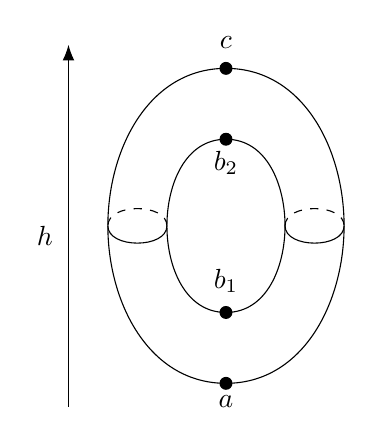
\begin{tikzpicture}
	%Draw the torus
	\draw [] (0,2) to [out=0,in=90] (1.5,0) to [out=270,in=0] (0,-2) to [out=180,in=270] (-1.5,0) to [out=90,in=180] (0,2);
	\draw [] (0.75,0) to [out=270,in=0] (0,-1.1) to [out=180,in=270] (-0.75,0) to [out=90,in=180] (0,1.1) to [out=0,in=90] (0.75,0);
	\draw [] (-1.5,0) to [out=270,in=270] (-0.75,0);
	\draw [dashed] (-0.75,0) to [out=90,in=90] (-1.5,0);
	\draw [] (1.5,0) to [out=270,in=270] (0.75,0);
	\draw [dashed] (0.75,0) to [out=90,in=90] (1.5,0);

	%Critical point c
	\draw [fill] (0,2) circle [radius=0.75mm]
	node [label={[above]$c$}] {};
	%Critical point b_2
	\draw [fill] (0,1.1) circle [radius=0.75mm]
	node [label={[below,yshift=-1.5mm]$b_2$}] {};
	%Critical point b_1
	\draw [fill] (0,-1.1) circle [radius=0.75mm]
	node [label={[above]$b_1$}] {};
	%Critical point a
	\draw [fill] (0,-2) circle [radius=0.75mm]
	node [label={[below,yshift=-1.5mm]$a$}] {};

	%Function h
	\draw [-{Latex[length=2mm]}] (-2,-2.3) to (-2,2.3);
	\draw (-2.3,-0.5) node [label={$h$}]{};
\end{tikzpicture}

		\caption{Critical points in the torus}
		\label{figure:torus1}
	\end{figure}
\end{frame}

\begin{frame}{Example (II)}
	Region under the hypersurface $h(x) = K$:

	\begin{figure}[h]
		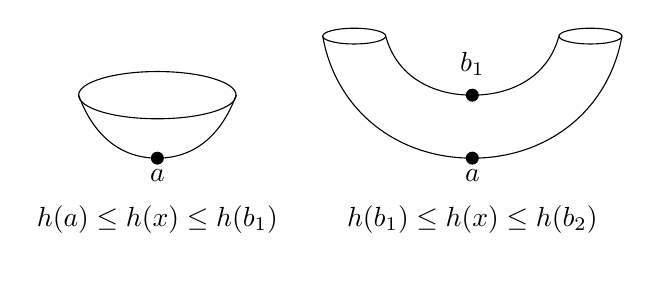
\begin{tikzpicture}
	%Figure at the left
	\draw (-2,0) ellipse (1cm and 3mm);
	%Connection
	\draw (-3,0) to [out=290,in=180] (-2,-0.8) to [out=0,in=250] (-1,0);
	%Critical point a
	\draw [fill] (-2,-0.8) circle [radius=0.75mm]
	node [label={[below,yshift=-1.5mm]$a$}] {};
	%Label of the region
	\draw (-2,-2) node [label={$h(a) \leq h(x) \leq h(b_1)$}]{};

	%Figure at the right
	%End circles of the cilinder
	\draw (0.5,0.75) ellipse (4mm and 1mm);
	\draw (3.5,0.75) ellipse (4mm and 1mm);
	\draw (0.9,0.75) to [out=285,in=180] (2,0) to [out=0,in=255] (3.1,0.75);
	\draw (0.1,0.75) to [out=280,in=180] (2,-0.8) to [out=0,in=260] (3.9,0.75);
	%Critical point b_1
	\draw [fill] (2,0) circle [radius=0.75mm]
	node [label={[above]$b_1$}] {};
	%Critical point a
	\draw [fill] (2,-0.8) circle [radius=0.75mm]
	node [label={[below,yshift=-1.5mm]$a$}] {};
	%Label of the region
	\draw (2,-2) node [label={$h(b_1) \leq h(x) \leq h(b_2)$}]{};
\end{tikzpicture}

		\caption{Formation of the torus}
		\label{figure:torus2}
	\end{figure}
\end{frame}

\begin{frame}{Example (III)}
	Region under the hypersurface $h(x) = K$:

	\begin{figure}[h]
		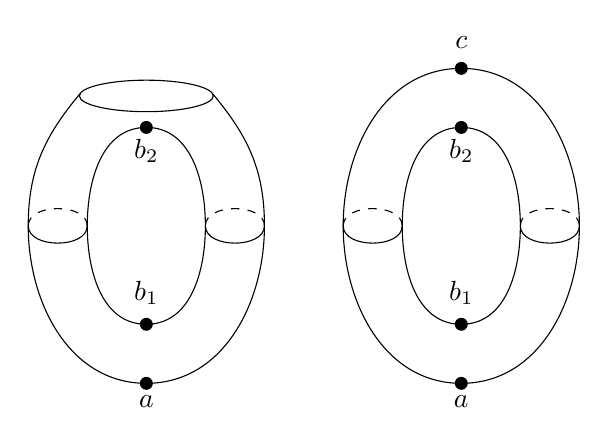
\begin{tikzpicture}
	%Figure at the left
	\draw [] (-1.16,1.68) to [out=310,in=90] (-0.5,0) to [out=270,in=0] (-2,-2) to [out=180,in=270] (-3.5,0) to [out=90,in=230] (-2.84,1.68);
	\draw [] (-1.25,0) to [out=270,in=0] (-2,-1.25) to [out=180,in=270] (-2.75,0) to [out=90,in=180] (-2,1.25) to [out=0,in=90] (-1.25,0);
	\draw [] (-0.5,0) to [out=270,in=270] (-1.25,0);
	\draw [dashed] (-0.5,0) to [out=90,in=90] (-1.25,0);
	\draw [] (-2.75,0) to [out=270,in=270] (-3.5,0);
	\draw [dashed] (-2.75,0) to [out=90,in=90] (-3.5,0);

	%Section at the top
	\draw (-2,1.65) ellipse (8.5mm and 2mm);

	%Critical point b_2
	\draw [fill] (-2,1.25) circle [radius=0.75mm]
	node [label={[below,yshift=-1.5mm]$b_2$}] {};
	%Critical point b_1
	\draw [fill] (-2,-1.25) circle [radius=0.75mm]
	node [label={[above]$b_1$}] {};
	%Critical point a
	\draw [fill] (-2,-2) circle [radius=0.75mm]
	node [label={[below,yshift=-1.5mm]$a$}] {};

	%Figure at the right (Torus)
	\draw [] (2,2) to [out=0,in=90] (3.5,0) to [out=270,in=0] (2,-2) to [out=180,in=270] (0.5,0) to [out=90,in=180] (2,2);
	\draw [] (2.75,0) to [out=270,in=0] (2,-1.25) to [out=180,in=270] (1.25,0) to [out=90,in=180] (2,1.25) to [out=0,in=90] (2.75,0);
	\draw [] (0.5,0) to [out=270,in=270] (1.25,0);
	\draw [dashed] (0.5,0) to [out=90,in=90] (1.25,0);
	\draw [] (2.75,0) to [out=270,in=270] (3.5,0);
	\draw [dashed] (2.75,0) to [out=90,in=90] (3.5,0);

	%Critical point c
	\draw [fill] (2,2) circle [radius=0.75mm]
	node [label={[above]$c$}] {};
	%Critical point b_2
	\draw [fill] (2,1.25) circle [radius=0.75mm]
	node [label={[below,yshift=-1.5mm]$b_2$}] {};
	%Critical point b_1
	\draw [fill] (2,-1.25) circle [radius=0.75mm]
	node [label={[above]$b_1$}] {};
	%Critical point a
	\draw [fill] (2,-2) circle [radius=0.75mm]
	node [label={[below,yshift=-1.5mm]$a$}] {};
\end{tikzpicture}

		\caption{Completion of the torus}
		\label{figure:torus3}
	\end{figure}
\end{frame}

\end{document}
